\documentclass[14pt]{extreport}

% Основные пакеты
\usepackage[english, russian]{babel}    % Поддержка русского и английского языков
\usepackage{graphicx}                   % Для вставки изображений
\usepackage{import}                     % Для продвинутого импорта (например, pdf_tex из Inkscape)
\usepackage{subcaption}                 % Для создания подписей к фигурам
\usepackage{float}                      % Для улучшенного позиционирования фигур
\usepackage{geometry}                   % Для управления отступами на странице
\usepackage{amsmath}                    % Для расширенной поддержки математики
\usepackage{amsfonts}                   % Математические шрифты
\usepackage{amssymb}                    % Математические символы
\usepackage{tabu}                       % Улучшенные таблицы
\usepackage{booktabs}                   % Профессиональные таблицы с вертикальными разделителями
\usepackage[dvipsnames]{xcolor}         % Расширенная поддержка цветов
\usepackage{longtable}                  % Для таблиц, занимающих несколько страниц
\usepackage{makecell}                   % Для улучшенного форматирования ячеек таблиц
\usepackage{multirow}                   % Для объединения строк в таблицах
\usepackage{tabularray}                 % Для современных таблиц
\usepackage{varwidth}                   % Для переменной ширины блоков
\usepackage{hyperref}                   % Для гиперссылок
\usepackage{verbatim}                   % Для вставки кода
\usepackage{listings}                   % Для оформления листингов кода
\usepackage{amsmath}
% Настройка графики
\graphicspath{ {./images/} }            % Путь к папке с изображениями

% Настройка отступов на странице
\geometry{left=2cm, right=2cm, bottom=2cm, top=2cm}

% Настройка гиперссылок
\hypersetup{
    linkcolor=blue,                     % Цвет ссылок
    filecolor=magenta,                  % Цвет ссылок на файлы
    urlcolor=cyan                       % Цвет URL-адресов
}

% Настройка листингов кода
\definecolor{codegreen}{rgb}{0,0.6,0}
\definecolor{codegray}{rgb}{0.5,0.5,0.5}
\definecolor{codepurple}{rgb}{0.58,0,0.82}
\definecolor{backcolour}{rgb}{0.95,0.95,0.92}

\lstdefinestyle{codestyle}{
    backgroundcolor=\color{backcolour},
    commentstyle=\color{codegreen},
    keywordstyle=\color{magenta},
    numberstyle=\tiny\color{codegray},
    stringstyle=\color{codepurple},
    basicstyle=\ttfamily\footnotesize,
    breakatwhitespace=false,
    breaklines=true,
    captionpos=b,
    keepspaces=true,
    numbers=left,
    numbersep=5pt,
    showspaces=false,
    showstringspaces=false,
    showtabs=false,
    tabsize=2
}

\lstset{style=codestyle}
\lstset{extendedchars=\true}

\begin{document}

\begin{titlepage}
    \centering
    \vspace*{1cm}

    {\large Министерство науки и высшего образования Российской Федерации}\\
    {\large ФЕДЕРАЛЬНОЕ ГОСУДАРСТВЕННОЕ АВТОНОМНОЕ ОБРАЗОВАТЕЛЬНОЕ УЧРЕЖДЕНИЕ ВЫСШЕГО ОБРАЗОВАНИЯ «НАЦИОНАЛЬНЫЙ ИССЛЕДОВАТЕЛЬСКИЙ УНИВЕРСИТЕТ ИТМО»}\\
    {\large (УНИВЕРСИТЕТ ИТМО)}\\

    \vspace{1cm}

    \textbf{{\Huge ОТЧЕТ}\\
    {\Huge О ЛАБОРАТОРНОЙ РАБОТЕ №1}}\\

    \vspace{1cm}

    {\LARGE По дисциплине\\
     \(\lll\) Математическая Статистика \(\ggg\) }\\

    \vspace{2cm}

    {\Large Студенты:}\\
    Охрименко Eва\\
    Даниил Буцкий


    \vspace{2cm}

    {\Large Проверил:}\\
    Шкваренко Андрей Алексеевич\\

    \vspace{2cm}

    {\large г. Санкт-Петербург}\\
    {\large 2025}

\end{titlepage}
\newpage
\tableofcontents
\newpage

\chapter{Задание 1}

\section{Выбор распределения и параметров}

Выбираем распределение, у которого существуют первые четыре момента. В нашем случае это нормальное распределение.

$\mu$ (мю) определяет центр нормального распределения на числовой оси. Это точка, вокруг которой группируются значения.

$\sigma$ (сигма) определяет "ширину" нормального распределения, то есть, насколько разбросаны значения относительно $\mu$.

\begin{verbatim}
# Параметры распределения
mu = 0       # Центр нормального распределения
sigma = 1    # Стандартное отклонение
\end{verbatim}

\section{Генерация выборок}

Генерируем достаточно большое количество выборок достаточно большого объема из выбранного распределения.

\begin{verbatim}
# Параметры генерации выборок
M = 10000     # Количество выборок
n = 1000      # Размер выборки

# Генерация выборок из нормального распределения
samples = np.random.normal(mu, sigma, size=(M, n))
\end{verbatim}

\textbf{Пояснение:}

\begin{itemize}
    \item $M$: Определяет, сколько раз мы будем повторять эксперимент (генерировать выборку и вычислять статистики).
    \item $n$: Определяет размер каждой выборки.
    \item \texttt{np.random.normal(mu, sigma, size=(M, n))}: Генерирует $M$ выборок размером $n$ из нормального распределения с параметрами $\mu$ и $\sigma$.
\end{itemize}

\section{Вычисление выборочных статистик}

Для каждой сгенерированной выборки вычисляем соответствующие статистики: выборочное среднее, выборочную дисперсию и выборочную медиану.

\begin{verbatim}
# Вычисление статистик для каждой выборки
means = np.mean(samples, axis=1)           # Выборочные средние
variances = np.var(samples, axis=1, ddof=1)  # Выборочные дисперсии
medians = np.median(samples, axis=1)         # Медианы
\end{verbatim}

Выборочное среднее $\bar{X}$ --- это среднее значение выборки $X_1, X_2, \dots, X_n$, вычисляемое по формуле:
\[
\bar{X} = \frac{1}{n} \sum_{i=1}^n X_i.
\]

Выборочная дисперсия $S^2$ --- это мера разброса значений выборки относительно выборочного среднего. Несмещенная оценка выборочной дисперсии вычисляется по формуле:
\[
S^2 = \frac{1}{n-1} \sum_{i=1}^n (X_i - \bar{X})^2.
\]

Квантиль порядка $p$ --- это значение, которое случайная величина не превышает с вероятностью $p$. Квантиль порядка $0.5$ называется медианой и является серединным значением в упорядоченной выборке.

\textbf{Пояснение:}

\begin{itemize}
    \item \texttt{np.mean(samples, axis=1)}: Вычисляет выборочное среднее для каждой выборки (среднее по строкам матрицы \texttt{samples}).
    \item \texttt{np.var(samples, axis=1, ddof=1)}: Вычисляет выборочную дисперсию для каждой выборки. \texttt{ddof=1} обеспечивает несмещенную оценку дисперсии.
    \item \texttt{np.median(samples, axis=1)}: Вычисляет медиану для каждой выборки.
\end{itemize}

\section{Построение гистограмм и наложение теоретической плотности}

Строим гистограммы результатов для каждой выборочной статистики. Для наглядности рядом с гистограммой рисуем соответствующую теоретическую плотность.

Асимптотическая нормальность означает, что при увеличении размера выборки ($n \to \infty$), распределение выборочной статистики сходится к нормальному распределению. Это важный результат, позволяющий использовать свойства нормального распределения для анализа статистик при больших выборках.

\begin{verbatim}
# Функция для построения гистограмм и наложения теоретической плотности
def plot_histogram(data, theoretical_dist, params, title):
    plt.hist(data, bins=30, density=True, alpha=0.6, color='blue', label='Гистограмма')
    x = np.linspace(min(data), max(data), 100)
    pdf = theoretical_dist.pdf(x, *params)
    plt.plot(x, pdf, 'r-', label='Теоретическая плотность')
    plt.legend()
    plt.title(title)
    plt.show()

# Гистограмма для выборочного среднего
plot_histogram(
    means,
    norm,
    (mu, sigma / np.sqrt(n)),
    'Выборочное среднее'
)

# Гистограмма для выборочной дисперсии
plot_histogram(
    variances,
    norm,
    (mu, sigma / np.sqrt(n)),
    'Выборочная дисперсия'
)

# Гистограмма для медианы
plot_histogram(
    medians,
    norm,
    (mu, sigma / np.sqrt(n)),
    'Медиана'
)
\end{verbatim}

\begin{figure}[H]
    \centering
    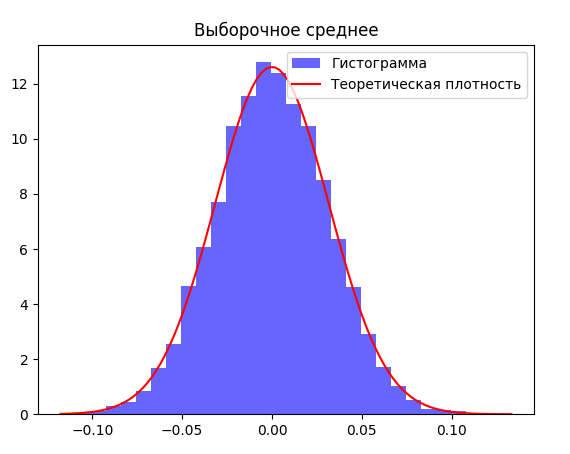
\includegraphics[width=0.9\linewidth]{1.png}
    \caption{Выборочное среднее}
\end{figure}

\begin{figure}[H]
    \centering
    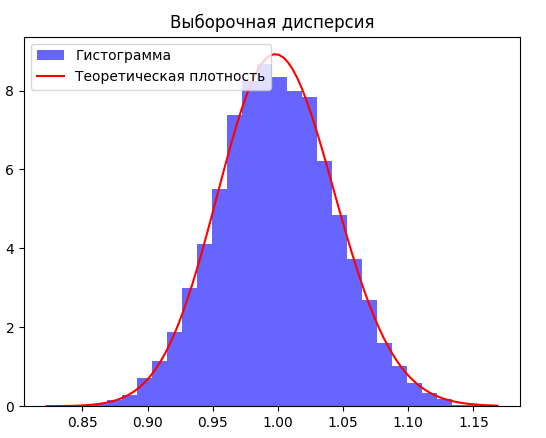
\includegraphics[width=0.9\linewidth]{2.png}
    \caption{Выборочная дисперсия}
\end{figure}

\begin{figure}[H]
    \centering
    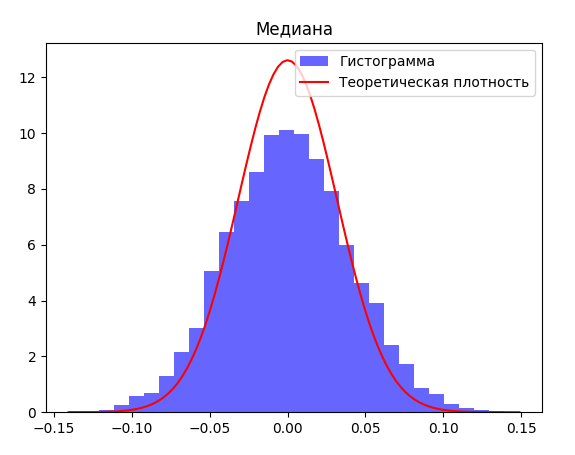
\includegraphics[width=0.9\linewidth]{3.png}
    \caption{Медиана}
\end{figure}

\section{Проверка сходимости $nF(X_{(2)})$ и $n(1 - F(X_{(n)}))$}

Экспериментально убеждаемся в том, что $nF(X_{(2)}) \to \Gamma(2, 1)$ и $n(1 - F(X_{(n)})) \to \Gamma(1, 1) = \text{Exp}(1)$.

\begin{verbatim}
# Проверка утверждений о U1 и U2
sorted_samples = np.sort(samples, axis=1)
X_2 = sorted_samples[:, 1]       # Второй элемент в каждой выборке
X_n = sorted_samples[:, -1]      # Максимальный элемент в каждой выборке

# Вычисление F(X) с помощью функции распределения нормального закона
F_X_2 = norm.cdf(X_2, loc=mu, scale=sigma)
F_X_n = norm.cdf(X_n, loc=mu, scale=sigma)

# Сходимость величин U_1 и U_2
U_1 = n * F_X_2                 # nF(X_(2))
U_2 = n * (1 - F_X_n)           # n(1 - F(X_(n)))

# Гистограмма для U_1 (Gamma(2, 1))
plot_histogram(
    U_1,
    gamma,
    (2,),  # Параметры гамма-распределения: shape=2
    'Сходимость U_1 к Gamma(2, 1)'
)

# Гистограмма для U_2 (Exp(1))
plot_histogram(
    U_2,
    expon,
    (),  # Параметры экспоненциального распределения: scale=1
    'Сходимость U_2 к Exp(1)'
)
\end{verbatim}

\begin{figure}[H]
    \centering
    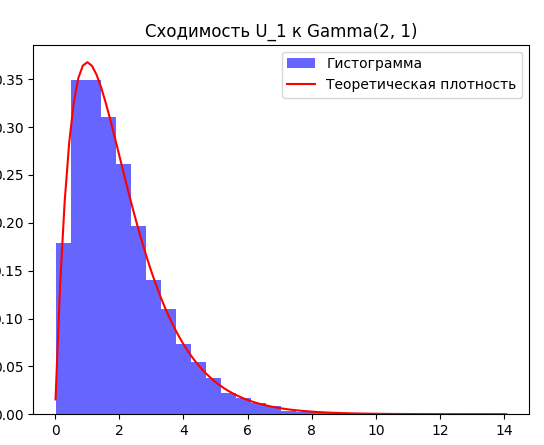
\includegraphics[width=0.9\linewidth]{4.png}
    \caption{Сходимость \(U_1\)}
\end{figure}

\begin{figure}[H]
    \centering
    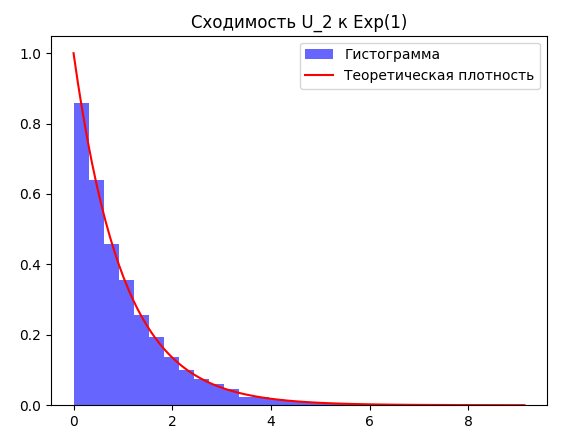
\includegraphics[width=0.9\linewidth]{5.png}
    \caption{Сходимость \(U_2\)}
\end{figure}

\section{Вывод статистик}

Выводим математическое ожидание и дисперсию каждой выборочной статистики для проверки согласованности с законом распределения.

\begin{verbatim}
# Вывод статистик
print("Мат. ожидание выборочного среднего:", np.mean(means))
print("Дисперсия выборочного среднего:", np.var(means))
print("Мат. ожидание выборочной дисперсии:", np.mean(variances))
print("Дисперсия выборочной дисперсии:", np.var(variances))
print("Мат. ожидание медианы:", np.mean(medians))
print("Дисперсия медианы:", np.var(medians))
print("Мат. ожидание U1:", np.mean(U_1))
print("Дисперсия U1:", np.var(U_1))
print("Мат. ожидание U2:", np.mean(U_2))
print("Дисперсия U2:", np.var(U_2))
\end{verbatim}

\begin{figure}[H]
    \centering
    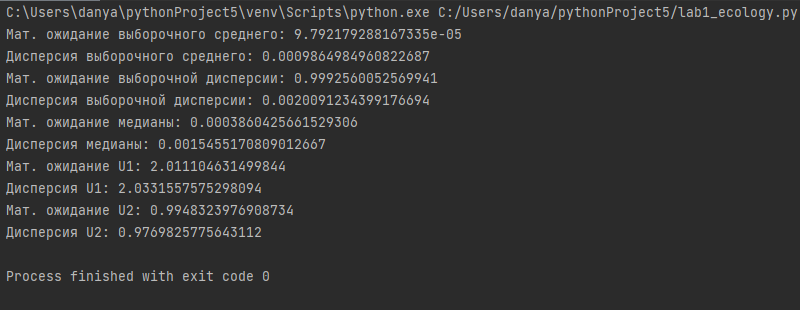
\includegraphics[width=0.9\linewidth]{6.png}
    \caption{Вывод статистик}
\end{figure}


\newpage
\chapter{Задание 2}
\section{Первые три вопроса}
    В этом задании нашей команде нужно было сделать 4 вариант.
Итак, для начала ответим на первые простые 3 вопроса: "Сколько моделей телефонов
можно вставить 2 сим-карты, сколько поддерживают 3G, каково наибольшее число ядер 
у процессора?". Для этого напишем код, который открывает наш файл и все считает:

\begin{lstlisting}[language=Python, caption={Код для первых трех вопросов}]
file = open("/home/eva/Документы/ITMO/2_course/MatStat/lab1/mobile_phones.csv")

counter = 0
data = list()

counterDualSim = 0
counterTreeG = 0
maxNCores = -100500

for str in file:
    counter += 1
    if counter != 1:
        row = (list(map(float, str.split(','))))
        data.append(row)

        if row[3] == True:
            counterDualSim += 1
        if row[-4] == True:
            counterTreeG += 1
        if row[9] > maxNCores:
            maxNCores = row[9]

print(counterDualSim, " - столько телефонов поддерживают 2 сим-карты")
print(counterTreeG, " - столько телефонов имеют 3G")
print(int(maxNCores), "- максимальное число ядер процессора")
\end{lstlisting}

Этот код в цикле вычленяет определенные значения и инкрементирует определенные 
\texttt{counter}. Также он ищет максимальное число ядер процессора. Посмотрим на вывод:


\begin{lstlisting}[language=Python, caption={Вывод для первых трех вопросов}]
1019  - столько телефонов поддерживают 2 сим-карты
1523  - столько телефонов имеют 3G
8 - максимальное число ядер процессора
\end{lstlisting}


\section{Написание остальных функций}

Далее по заданию нужно расчитать несколько параметров для наших выборок.
Выборки - это 3 массива данных, в них будет содержаться информация о емкости
аккумулятора для всей совокупности, для телефонов, поддерживающих Wi-Fi и для
телефонов, не поддерживающих Wi-Fi.
Упустим то, как мы из двумерного массива нашли 3 нам подходящих и передем к написанию функций:\\

\subsubsection{Функция выборочного среднего}
1 функция - функция выборочного среднего. Мы ее находили по формуле:

\[
\bar{X} = \frac{1}{n} \sum_{i=1}^{n} x_i
\]

\begin{lstlisting}[language=Python, caption={Функция поиска выборочного среднего}]
def calculateMean(data):
    return sum(data) / len(data)
\end{lstlisting}



\subsubsection{Выборочная дисперсия}
Эту функцию мы считали по формуле:

\[
\sigma^2 = \frac{1}{n-1} \sum_{i=1}^{n} (x_i - \bar{X})^2
\]

\begin{lstlisting}[language=Python, caption={Функция поиска выборочной дисперсии}]
def calculateVariance(data):
    mean = calculateMean(data)
    return sum((x - mean) ** 2 for x in data) / (len(data) - 1)
\end{lstlisting}

\subsubsection{Выборочная медиана}
Ее мы считали по формуле:
\[
E = 
\begin{cases}
x_{k}, & \text{если } n \text{ нечётное}, \\
\frac{x_{k} + x_{k+1}}{2}, & \text{если } n \text{ чётное},
\end{cases}
\]
где \( k = \left\lfloor \frac{n}{2} \right\rfloor + 1 \).

\begin{lstlisting}[language=Python, caption={Функция поиска выборочной медианы}]
def calculateMedian(data):
    sortedData = sorted(data)
    n = len(sortedData)
    if n % 2 == 1:
        return sortedData[n // 2]
    else:
        return (sortedData[n // 2 - 1] + sortedData[n // 2]) / 2
\end{lstlisting}

\subsubsection{Выборочный квантиль порядка \(\frac{2}{5}\)}
\[
Q_p = x_{\lfloor i \rfloor} + (i - \lfloor i \rfloor) \cdot (x_{\lfloor i \rfloor + 1} - x_{\lfloor i \rfloor}),
\]
где \( i = p \cdot (n - 1) \).

\begin{lstlisting}[language=Python, caption={Функция поиска выборочного квантиля порядка \(\frac{2}{5}\)}]
def calculateQuantile(data, p):
    sortedData = sorted(data)
    n = len(sortedData)
    index = p * (n - 1)
    lowerIndex = int(index)
    fraction = index - lowerIndex
    if lowerIndex + 1 < n:
        return sortedData[lowerIndex] + fraction * (sortedData[lowerIndex + 1] - sortedData[lowerIndex])
    return sortedData[lowerIndex]
\end{lstlisting}

\subsubsection{Графики}
А также мы построим для наших выборок графики эмпирической функции распределения,
гистограмму и box-plot (в одной функции, чтобы все графики поместились на одной фигуре).

\begin{lstlisting}[language=Python, caption={Графики распределения}]
def plots(data, title="Графики распределения"):

    fig, axes = plt.subplots(1, 3, figsize=(18, 6))
    fig.suptitle(title, fontsize=16)

    sorted_data = sorted(data)
    n = len(sorted_data)
    x_values = sorted_data
    y_values = [i / n for i in range(1, n + 1)]
    
    axes[0].step(x_values, y_values, where='post', label='ЭФР', color='red', linewidth=2.5)
    axes[0].set_xlabel('Значения', fontsize=12)
    axes[0].set_ylabel('F(x)', fontsize=12)
    axes[0].set_title('Эмпирическая функция распределения', fontsize=14)
    axes[0].legend(fontsize=10)
    axes[0].grid(True)

    axes[1].hist(data, bins=30, color='blue', edgecolor='black', linewidth=1.5)
    axes[1].set_xlabel('Значения', fontsize=12)
    axes[1].set_ylabel('Частота', fontsize=12)
    axes[1].set_title('Гистограмма', fontsize=14)
    axes[1].grid(True)

    axes[2].boxplot(data, vert=True, patch_artist=True, boxprops=dict(facecolor="lightblue"))
    axes[2].set_ylabel('Значения', fontsize=12)
    axes[2].set_title('Box-plot', fontsize=14)
    axes[2].grid(True)
    
    plt.tight_layout()
    plt.show()
\end{lstlisting}

\section{Выводы по написанным функциям}
Итак теперь посмотрим, что выведет наш код для разных выборок:

\subsection*{Выводы по емкости аккумуляторя для всех телефонов}

\begin{lstlisting}[language=Python, caption={Вывод 1}]
1238.5185 - выборочное среднее
193088.35983766866 - выборочная дисперсия
1226.0 - выборочная медиана
1076.0 - выборочная квантиль порядка 2/5
\end{lstlisting}

\begin{figure}[H]
    \centering
    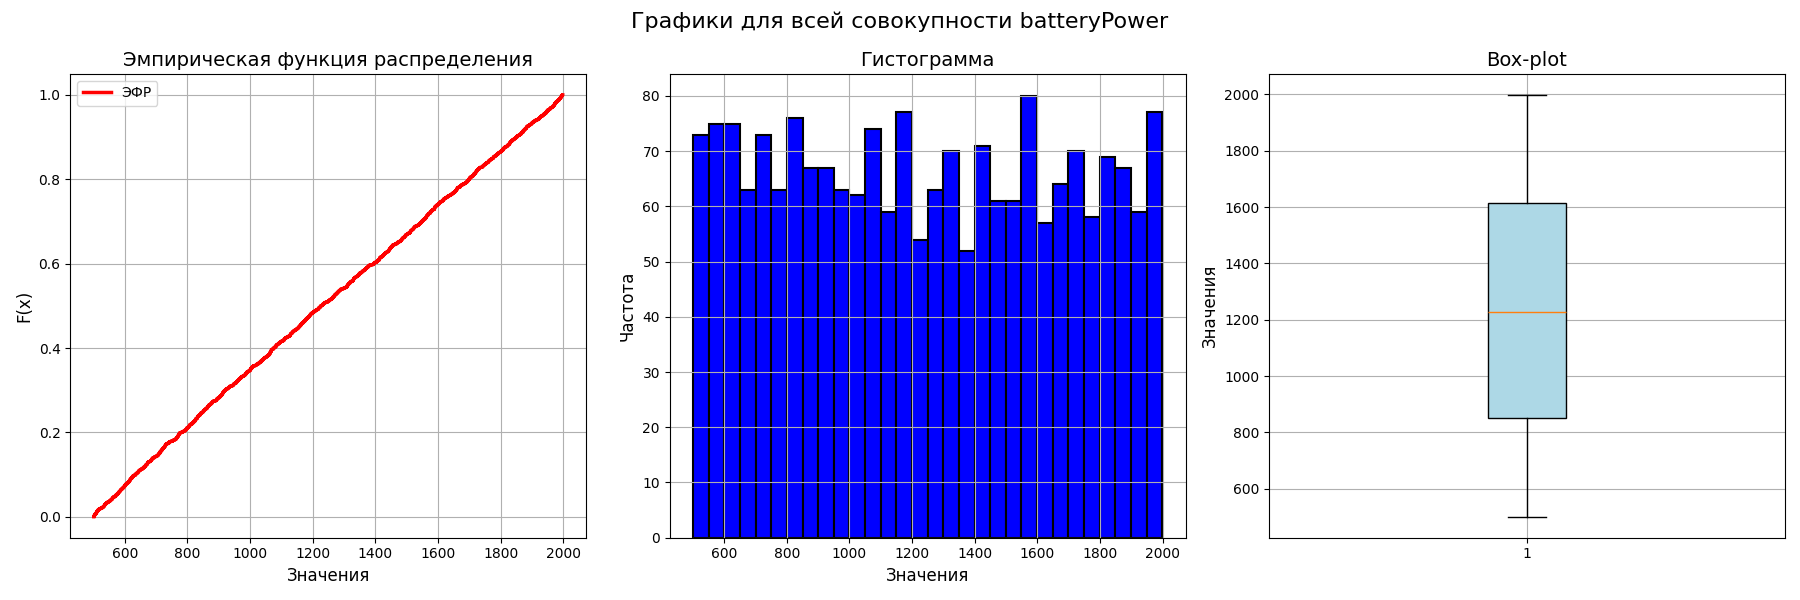
\includegraphics[width=1\linewidth]{Figure_1.png}
    \caption{Графики 1}
\end{figure}


\subsection*{Выводы по емкости аккумуляторя для телефонов с Wi-Fi}

\begin{lstlisting}[language=Python, caption={Вывод 2}]
1234.9043392504932 - выборочное среднее
190296.40051422257 - выборочная дисперсия
1233.0 - выборочная медиана
1077.8000000000002 - выборочная квантиль порядка 2/5
\end{lstlisting}

\begin{figure}[H]
    \centering
    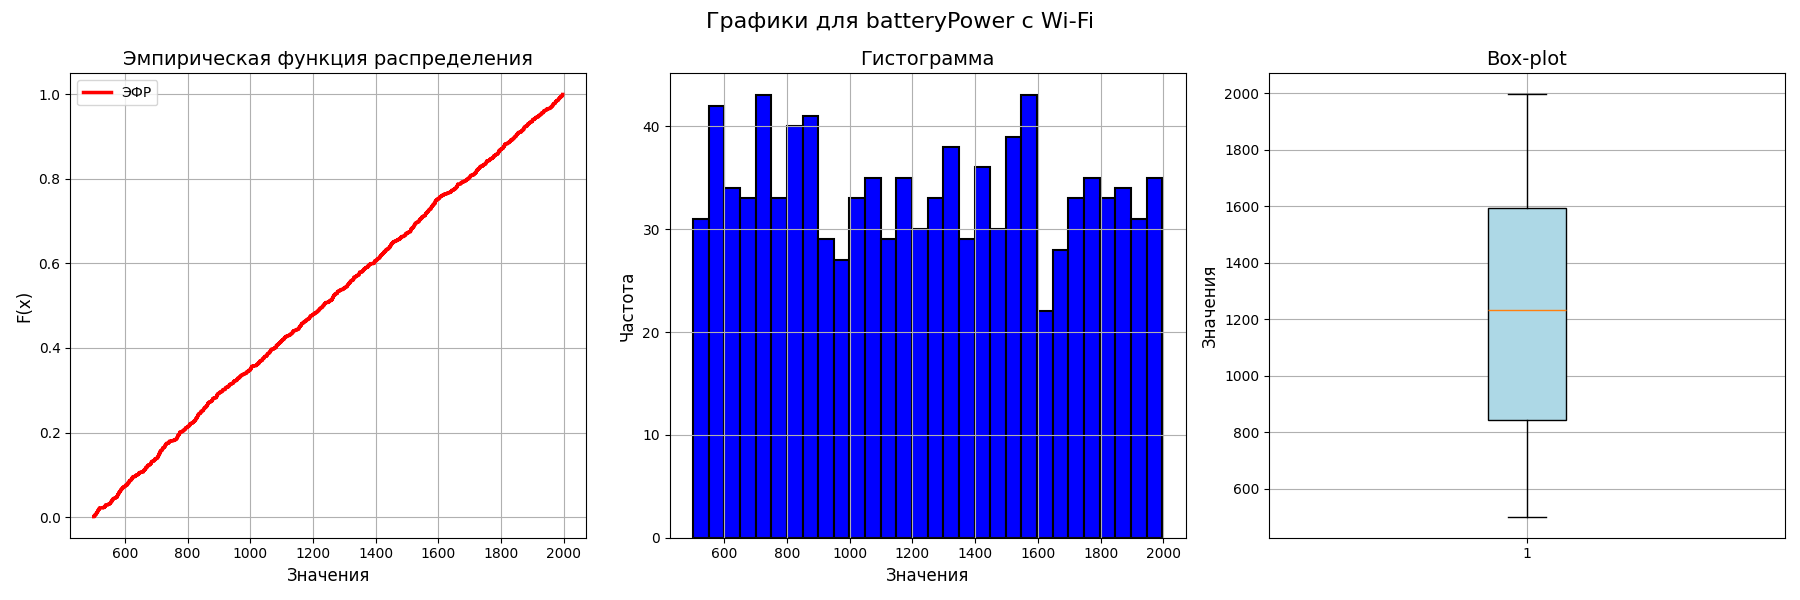
\includegraphics[width=1\linewidth]{Figure_2.png}
    \caption{Графики 2}
\end{figure}

\subsection*{Выводы по емкости аккумуляторя для телефонов без Wi-Fi}

\begin{lstlisting}[language=Python, caption={Вывод 3}]
1242.235294117647 - выборочное среднее
196128.43798148725 - выборочная дисперсия
1222.0 - выборочная медиана
1076.0 - выборочная квантиль порядка 2/5
\end{lstlisting}

\begin{figure}[H]
    \centering
    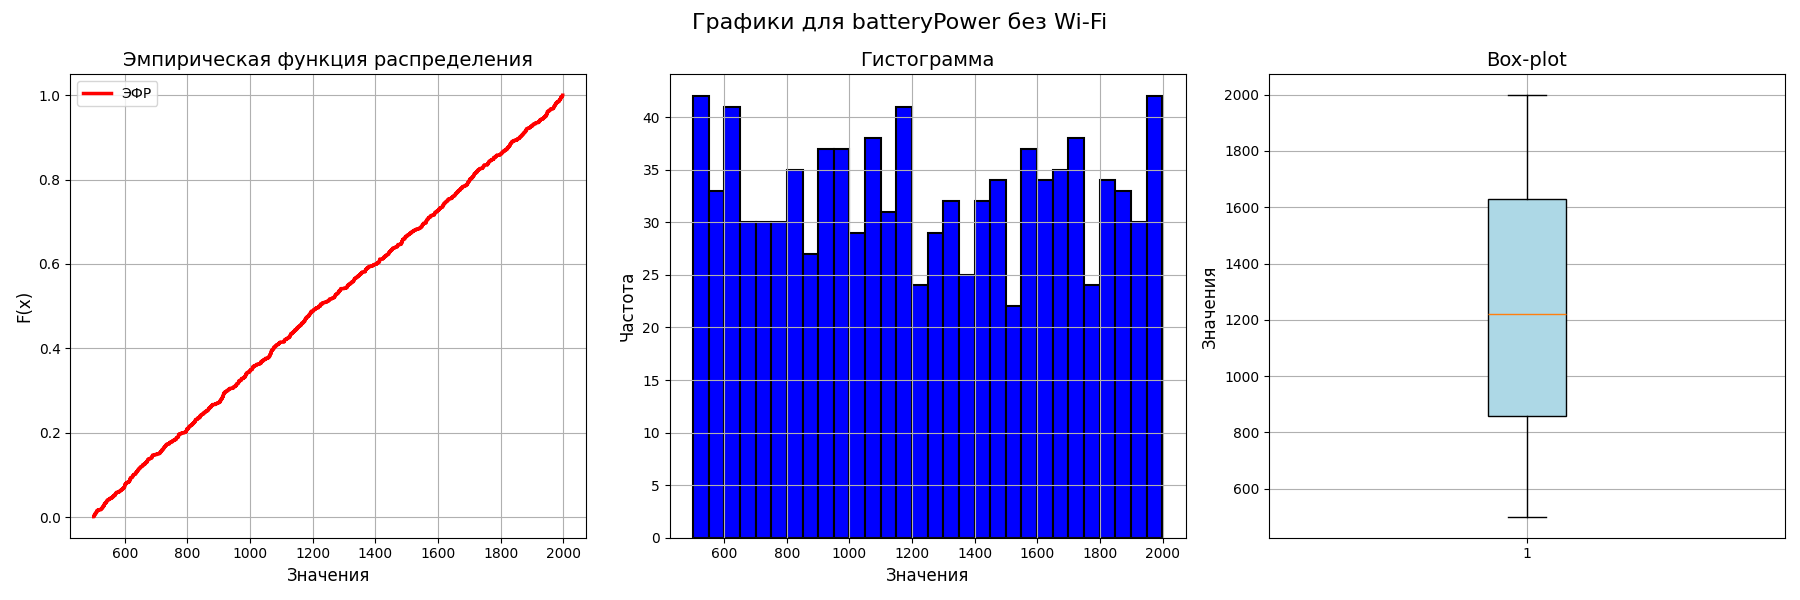
\includegraphics[width=1\linewidth]{Figure_3.png}
    \caption{Графики 3}
\end{figure}


\end{document}